% id: 173-353
% book: 개념원리 기하 · 21 위치벡터
% section: 필수·발전 예제
% figure: crop:fig-173-353.png
% answer: $p=\dfrac{1}{3}$, $q=\dfrac{1}{3}$, $r=-1$
% answer_source: 답지
% variant_level: 0 (원본 전사)
% 이 파일은 build.mjs 가 items.json 에서 만든다. 고칠 때는 items.json 을 고친다.
\smash{\raisebox{1.5mm}{\dmkichul{개념원리 기하 173쪽 353번 · 확인체크}}}
\noindent\begin{minipage}[t]{0.58\linewidth}\vspace{0pt}\raggedright 오른쪽 그림과 같은 정사면체~$\pt{OABC}$에서 삼각형~$\pt{OAB}$의 무게중심을 $\pt{G}$라 하고 $\vecAB{OA}=\vec{a}$, $\vecAB{OB}=\vec{b}$, $\vecAB{OC}=\vec{c}$라 할 때, $\vecAB{CG}=p\vec{a}+q\vec{b}+r\vec{c}$이다. 이때 실수 $p$, $q$, $r$의 값을 구하시오.\end{minipage}\hfill\begin{minipage}[t]{0.4\linewidth}\vspace{0pt}\centering \setlength{\dmfigw}{88.5pt}\ifdim\dmfigw>\linewidth\setlength{\dmfigw}{\linewidth}\fi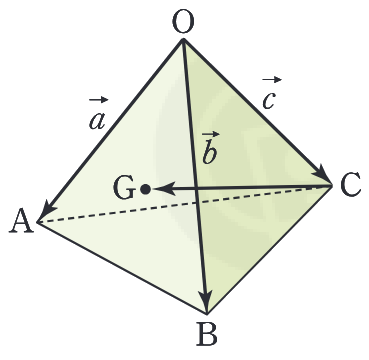
\includegraphics[width=\dmfigw]{figures/fig-173-353.png}\end{minipage}\par
